\documentclass[aip,pof,reprint,amsmath,amssymb,nofootinbib]{revtex4-2}

\usepackage[utf8]{inputenc}
\usepackage[T1]{fontenc}
\DeclareUnicodeCharacter{03BC}{\ensuremath{\mu}}
\usepackage{graphicx}
\usepackage{bm}
\usepackage{mathtools}
\usepackage{amsthm}
\usepackage{booktabs}
\usepackage{multirow}
\usepackage{algpseudocode}
\usepackage{xcolor}
\usepackage[colorlinks=true,linkcolor=blue!50!black,citecolor=blue!50!black,urlcolor=blue!50!black]{hyperref}
\usepackage[capitalise,nameinlink]{cleveref}

\newcommand{\TODO}[1]{\textcolor{red}{[TODO: #1]}}
\newcommand{\figplaceholder}[1]{\fbox{\parbox[c][0.28\textwidth][c]{0.9\linewidth}{\centering\small #1}}}

\theoremstyle{plain}
\newtheorem{theorem}{Theorem}
\newtheorem{lemma}{Lemma}
\newtheorem{proposition}{Proposition}
\newtheorem{corollary}{Corollary}
\theoremstyle{definition}
\newtheorem{definition}{Definition}
\newtheorem{assumption}{Assumption}
\theoremstyle{remark}
\newtheorem{remark}{Remark}
\crefname{assumption}{Assumption}{Assumptions}
\newcounter{algorithm}
\crefname{algorithm}{Algorithm}{Algorithms}
\Crefname{algorithm}{Algorithm}{Algorithms}

% ---- notation ----
\newcommand{\Wo}{\mathrm{Wo}}
\newcommand{\bu}{\bm{u}}
\newcommand{\bU}{\bm{U}}
\newcommand{\be}{\bm{e}}
\newcommand{\bx}{\bm{x}}
\newcommand{\bn}{\bm{n}}
\newcommand{\bF}{\bm{F}}
\newcommand{\bsig}{\bm{\sigma}}
\newcommand{\bI}{\bm{I}}
\newcommand{\bk}{\bm{k}}
\newcommand{\bM}{\mathsf{M}}
\newcommand{\dd}{\mathrm{d}}
\newcommand{\curl}{\nabla\times}

\begin{document}

% ------------------------------------------------------------------
% Candidate titles (stage 3, see notes/title_options.md)
% 1. Oscillatory hydrodynamics of a soft core--shell particle near a fluid--porous interface with stress jump  [CHOSEN]
% 2. Unsteady Stokes--Brinkman reflection theory for a core--shell sphere oscillating near a permeable biological layer
% 3. Porous walls shift and suppress the added-mass crossover of an oscillating soft particle
% 4. How does a permeable biological interface modify the frequency-dependent drag and added mass of a nearby soft cell or vesicle?
% 5. Hearing the glycocalyx: frequency-dependent drag and added mass of a soft particle oscillating near a Brinkman interface
% ------------------------------------------------------------------
\title{Oscillatory hydrodynamics of a soft core--shell particle near a fluid--porous interface with stress jump}

\author{Baraa A. Ahmed}
\email{\TODO{corresponding e-mail}}
\affiliation{\TODO{affiliation}}
\TODO{confirm author list and order}

\date{\today}

\begin{abstract}
% Guide bullets: the authors turn these into the final abstract (Physics of Fluids: single paragraph, <= 250 words).
\begin{itemize}
  \item \textbf{Context:} colloidal probes, cells and vesicles oscillate (AFM, acoustofluidics) next to permeable
        biological layers such as the endothelial glycocalyx and mucus; the frequency-dependent force carries information
        on both the particle and the layer.
  \item \textbf{Gap:} the unsteady force has been resolved only for a rigid sphere near a rigid wall; the porous
        layer (Brinkman, Ochoa-Tapia--Whitaker stress jump) and the soft (permeable-shell) particle have not been treated.
  \item \textbf{What we do:} semi-analytical solution of the unsteady Stokes--Brinkman problem for a core--shell sphere
        oscillating normal or parallel to a Brinkman half-space: exact sphere response, exact Fourier-space reflection at
        the porous interface, self-consistent dipolar closure summing all reflections; validated against
        exact and asymptotic limits.
  \item \textbf{Key results:} the wall-induced added mass changes sign at $\Wo_c\approx 2.9$ (normal) and $\approx 0.95$
        (parallel) near a rigid wall at $\varepsilon=1$; a permeable layer raises $\Wo_c$, opens an upper crossover at $\Wo\approx0.116\,\alpha_p^2$ beyond which the layer becomes hydrodynamically transparent, and below a threshold ($\alpha_p\approx6$--$9$ normal, $4$--$6$ parallel) removes the positive-added-mass window altogether; soft shells shift $\Wo_c$ non-monotonically and can remove it.
  \item \textbf{Implication:} a frequency sweep of the near-wall force is a non-contact spectroscopy of layer
        permeability and particle softness, relevant to glycocalyx microrheology, acoustofluidic CTC sorting and
        mucus-penetrating carriers.
\end{itemize}
% Draft paragraph (to be refined by the authors):
% Oscillating colloidal probes, cells and vesicles near permeable biological layers experience a frequency-dependent
% hydrodynamic force whose dissipative and inertial parts encode both particle and layer properties. We solve the
% unsteady Stokes--Brinkman problem for a core--shell sphere, with a Brinkman shell, a Navier-slip core and a stress-jump
% surface, oscillating normal or parallel to a semi-infinite Brinkman medium with an Ochoa-Tapia--Whitaker stress jump.
% The method combines the exact response of the sphere with an exact Fourier-space reflection of its unsteady
% singularities at the porous interface and a self-consistent dipolar closure that sums all orders of reflection. It
% reproduces the exact unsteady drag of rigid and porous spheres, Brenner's and Faxen's steady wall corrections and the
% inviscid image added mass. Near a rigid wall the wall-induced added mass changes sign at a critical Womersley number,
% as observed in recent AFM experiments. A permeable layer raises this crossover, introduces a second crossover beyond
% which the layer becomes hydrodynamically transparent, and for sufficiently permeable layers suppresses the
% positive-added-mass window entirely; particle softness shifts the crossover non-monotonically. These signatures
% suggest a non-contact spectroscopy of glycocalyx and mucus permeability and inform acoustofluidic sorting of cells
% that differ in softness.

\end{abstract}

\maketitle

\section{Introduction}\label{sec:intro}
% GUIDE POINTS ONLY -- the authors write the prose of this section.

\subsection*{Motivation: oscillating particles next to permeable biological layers}
\begin{itemize}
  \item Blood vessels are lined by the endothelial glycocalyx, a hydrodynamically relevant porous surface layer
        (near-wall $\mu$-PIV evidence~\cite{smith2003near}); airway and intestinal surfaces are covered by mucus
        that acts as a permeable barrier to particles and carriers~\cite{pangeni2023airway}.
  \item Particles near these layers are often driven harmonically: colloidal-probe AFM in dynamic mode
        (non-contact microrheology), and acoustofluidic devices that sort circulating tumour cells (CTCs) from
        leukocytes at $\Wo=O(1\text{--}10)$~\cite{wu2019acoustofluidic,hossein2023review}.
  \item Cells, liposomes and PEGylated carriers are hydrodynamically ``soft'': a permeable polymer or glycocalyx-like
        shell around a less permeable core. Both the particle and the wall are therefore porous.
  \item Key question: how do the permeability and interfacial stress jump of the layer, and the softness of the particle,
        reshape the frequency-dependent damping, added mass and phase lag of the near-wall force?
\end{itemize}

\subsection*{Unsteady hydrodynamics of a particle near a boundary}
\begin{itemize}
  \item Zhang \emph{et al.}~\cite{zhang2023unsteady}: rigid sphere oscillating normal to a rigid wall (FEM, asymptotics,
        thermal-noise AFM); in-phase and out-of-phase forces depend strongly on $\Wo$; the resonance-frequency shift
        crosses from positive to negative as $\Wo$ increases --- the benchmark generalised here.
  \item Point-particle and method-of-reflections theories for unsteady Stokes flow near walls~\cite{simha2018unsteady};
        generalised Faxén law for unsteady flow~\cite{mazur1974generalization}.
  \item Recent extensions: elastic (deformable) walls in the lubrication regime~\cite{batalha2026elasto};
        impermeable slip walls~\cite{elsapa2022force}; oscillation near a fluid--fluid interface~\cite{faltas2024oscillations}.
  \item Classical steady limits: Brenner~\cite{brenner1961slow} (normal) and Goldman--Cox--Brenner~\cite{goldman1967slow}
        (parallel).
\end{itemize}

\subsection*{Fluid--porous interfaces and porous particles}
\begin{itemize}
  \item Interface conditions: Beavers--Joseph slip~\cite{beavers1967boundary}; Ochoa-Tapia--Whitaker stress
        jump~\cite{ochoatapia1995momentum}; Brinkman model~\cite{brinkman1949calculation}.
  \item Unsteady flow next to a porous wall (no particle): Sherwood~\cite{sherwood2020unsteady}.
  \item Steady particle motion near a Brinkman interface with stress jump~\cite{faltas2021axisymmetric} and near a plane
        interface~\cite{richardson1996low}; Brinkman Green's functions near walls and plates~\cite{daddimoussaider2023axisymmetric,daddimoussaider2026asymptotic}.
  \item Oscillating porous particles in unbounded fluid~\cite{prakash2011arbitrary,ollila2012hydrodynamic}; oscillating spheres in
        Brinkman media~\cite{algatheem2025interaction}; Brinkman porous sphere with Beavers--Joseph slip~\cite{elsayed2026effect}.
\end{itemize}

\subsection*{Gap}
\begin{itemize}
  \item No study treats a finite-size particle oscillating near a \emph{permeable} half-space, nor a soft core--shell
        particle oscillating near any wall; the frequency signature of wall permeability and stress jump is unknown.
  \item Steady theories~\cite{faltas2021axisymmetric} miss inertia (added mass, Basset-type memory, phase lag); rigid-wall unsteady
        theories~\cite{zhang2023unsteady} miss permeability, which is the property of interest in biology.
\end{itemize}

\subsection*{Contributions}
\begin{itemize}
  \item A semi-analytical solution of unsteady Stokes--Brinkman flow for a core--shell sphere (Brinkman shell, Navier-slip
        core, OTW stress jump) oscillating normal or parallel to a Brinkman half-space with stress jump. It combines exact
        $l=1$ sphere solutions, an exact Fourier-space reflection of the unsteady singularities at the porous interface and
        a self-consistent dipolar closure that sums all orders of reflection (\cref{sec:analysis}).
  \item Validation against the exact unsteady drag of rigid and porous spheres, Brenner's and Faxén's steady wall
        corrections, and the inviscid image added mass, with a quantified accuracy envelope (\cref{sec:validation}).
  \item Maps of the interaction damping $\gamma_{\rm int}$, the added-mass shift $m_{\rm int}$ and the crossover Womersley
        numbers against $\alpha_p$, $\beta_p$, $\alpha_s$ and $\gamma$, for normal and parallel oscillation: permeable
        layers raise the lower crossover, create an upper crossover at $\Wo\approx0.116\,\alpha_p^2$, and can remove the
        positive-added-mass window (\cref{sec:results}).
  \item Bio-relevant consequences: non-contact estimation of glycocalyx or mucus permeability, force- and phase-contrast
        between cell-like particles of different softness, and design guidance for mucus-penetrating vesicles.
\end{itemize}

\subsection*{Organisation}
\begin{itemize}
  \item \cref{sec:formulation}: problem formulation; \cref{sec:analysis}: solution method and limiting cases;
        \cref{sec:results}: validation, parametric results and biomedical implications; \cref{sec:conclusion}: conclusions;
        appendix: radial functions and the interface system.
\end{itemize}

\section{Problem Formulation}\label{sec:formulation}

\subsection{Geometry and kinematics}\label{sec:geometry}
We consider a spherical core--shell particle of outer radius $b$ whose concentric, impermeable core has radius
$a=\gamma b$, $0\le\gamma\le1$ (\cref{fig:schematic}). The limit $\gamma=0$ is a homogeneous porous sphere and
$\gamma=1$ an impermeable sphere. The particle is immersed in an incompressible Newtonian fluid of density $\rho$ and
viscosity $\mu$ that fills the half-space $z>0$ (domain 1, outside $r=b$). The half-space $z<0$ (domain 3) is a
homogeneous, isotropic, rigid and stationary porous medium of permeability $k_p$ and Brinkman (effective) viscosity
$\mu_p$, saturated with the same fluid; it models a glycocalyx or mucus layer whose thickness exceeds the range of the
disturbance. The shell $a<r<b$ (domain 2) is a porous medium of permeability $k_s$ and Brinkman viscosity $\mu_s$.
The particle centre is at $\bx_0=h\be_z$ with $h>b$, and we write $r=|\bx-\bx_0|$, with $(r,\theta,\varphi)$ spherical
coordinates centred at $\bx_0$. The dimensionless gap is
\begin{equation}
  \varepsilon=\frac{h-b}{b}.\label{eq:gap}
\end{equation}
The particle translates without rotating at the velocity
\begin{equation}
  \bU(t)=\operatorname{Re}\!\left[U\be\,e^{-i\omega t}\right],\qquad
  \be=\be_z\ \text{(normal oscillation)}\quad\text{or}\quad\be=\be_x\ \text{(parallel oscillation)},
  \label{eq:kinematics}
\end{equation}
with angular frequency $\omega$ and complex amplitude $U$. All fields are written as
$\bu(\bx,t)=\operatorname{Re}[\bu(\bx)e^{-i\omega t}]$ and $p(\bx,t)=\operatorname{Re}[p(\bx)e^{-i\omega t}]$; we use the
same symbol for a field and its complex amplitude.

\begin{figure}[t]
  \centering
  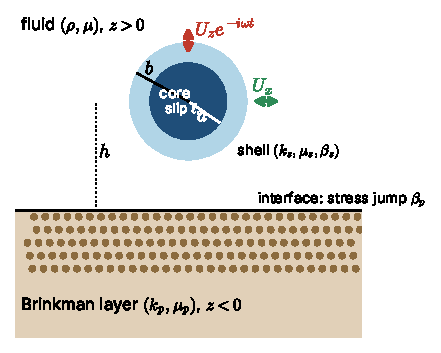
\includegraphics[width=0.8\linewidth]{figures/fig1_schematic.pdf}
  \caption{Core--shell particle (impermeable core of radius $a$ with Navier slip $\ell_c$; Brinkman shell of
  permeability $k_s$, viscosity $\mu_s$ and surface stress-jump coefficient $\beta_s$) oscillating with velocity
  $U\be\,e^{-i\omega t}$, normal ($\be_z$) or parallel ($\be_x$), at centre height $h$ above a semi-infinite Brinkman
  layer of permeability $k_p$ and viscosity $\mu_p$, coupled to the clear fluid through a stress-jump condition with
  coefficient $\beta_p$.}
  \label{fig:schematic}
\end{figure}

\subsection{Modelling assumptions}\label{sec:assumptions}
\begin{assumption}[Small amplitude]\label{as:linear}
The displacement amplitude $|U|/\omega$ is small compared with $b$ and with the gap $h-b$. Convective inertia
$\rho(\bu\cdot\nabla)\bu$ is then negligible relative to the unsteady inertia $\rho\,\partial_t\bu$, and all boundary
conditions are imposed at the mean particle position. The problem is linear and time-harmonic.
\end{assumption}
\begin{assumption}[Rigid porous matrices]\label{as:rigid}
The solid matrices of the shell and the layer are rigid: the shell matrix moves with the particle and the layer matrix
is at rest. Elastic deformation, which is the subject of
Ref.~\onlinecite{batalha2026elasto}, is not considered. ``Soft'' refers to hydrodynamic permeability, as in
soft-particle electrokinetics.
\end{assumption}
\begin{assumption}[Brinkman description]\label{as:brinkman}
Flow in each porous region obeys the unsteady Brinkman equation with Darcy drag relative to the local matrix. The
interfacial momentum transfer at both fluid--porous interfaces follows the Ochoa-Tapia--Whitaker (OTW) stress
jump~\cite{ochoatapia1995momentum}. The Beavers--Joseph slip model~\cite{beavers1967boundary} is recovered from the same
equations as the limit of a Darcy-dominated porous side (\cref{rem:bj}).
\end{assumption}
\begin{assumption}[Prescribed translation]\label{as:norotation}
The particle is driven in pure translation (an AFM colloidal probe glued to a cantilever, or a particle in an imposed
acoustic field), so no torque-free rotation is allowed. Translation--rotation coupling near a wall enters the force at
higher order in $b/h$ than is retained in \cref{sec:closure}.
\end{assumption}
\begin{assumption}[Thick layer]\label{as:thick}
The porous layer is modelled as a half-space. This is appropriate when its thickness exceeds both the Brinkman
screening length $\sqrt{k_p\mu_p/\mu}$ and the distance $h$, so that the reflected disturbance does not feel the
underlying substrate.
\end{assumption}

\subsection{Governing equations}\label{sec:equations}
In the clear fluid (domain 1) the unsteady Stokes equations hold:
\begin{equation}
  -i\omega\rho\,\bu^{(1)}=-\nabla p^{(1)}+\mu\nabla^2\bu^{(1)},\qquad\nabla\cdot\bu^{(1)}=0 .
  \label{eq:stokes}
\end{equation}
In the shell (domain 2) the Darcy drag acts on the velocity relative to the moving matrix:
\begin{equation}
  -i\omega\rho\,\bu^{(2)}=-\nabla p^{(2)}+\mu_s\nabla^2\bu^{(2)}-\frac{\mu}{k_s}\left(\bu^{(2)}-U\be\right),
  \qquad\nabla\cdot\bu^{(2)}=0 .
  \label{eq:shell}
\end{equation}
In the porous layer (domain 3),
\begin{equation}
  -i\omega\rho\,\bu^{(3)}=-\nabla p^{(3)}+\mu_p\nabla^2\bu^{(3)}-\frac{\mu}{k_p}\bu^{(3)},
  \qquad\nabla\cdot\bu^{(3)}=0 .
  \label{eq:layer}
\end{equation}
Taking the curl of \cref{eq:stokes,eq:shell,eq:layer} shows that the vorticity in each domain obeys a modified Helmholtz
equation $(\nabla^2-\lambda_j^2)\,\curl\bu^{(j)}=\bm 0$ with the complex screening parameters
\begin{equation}
  \lambda_f^2=-\frac{i\omega\rho}{\mu},\qquad
  \lambda_s^2=\frac{\mu/k_s-i\omega\rho}{\mu_s},\qquad
  \lambda_p^2=\frac{\mu/k_p-i\omega\rho}{\mu_p},
  \qquad\operatorname{Re}\lambda_j>0 .
  \label{eq:lambdas}
\end{equation}
The real part of $1/\lambda_f$ is the viscous penetration depth $\delta_v=\sqrt{2\mu/\rho\omega}$. Inside the porous
media the vortical disturbance is screened by both the Darcy drag and the unsteady inertia; whichever dominates sets
the decay length.

The stress tensor in domain $j$ is $\bsig^{(j)}=-p^{(j)}\bI+\mu_j(\nabla\bu^{(j)}+\nabla\bu^{(j)\mathsf T})$ with
$\mu_1=\mu$, $\mu_2=\mu_s$, $\mu_3=\mu_p$.

\subsection{Boundary and interface conditions}\label{sec:bcs}
Let $\bn$ be the outward unit normal of the relevant sphere and $\bm\Pi=\bI-\bn\bn$ the tangential projector.

\emph{Core surface} $r=a$ (impermeability and Navier slip of length $\ell_c$):
\begin{equation}
  \left(\bu^{(2)}-U\be\right)\cdot\bn=0,\qquad
  \bm\Pi\cdot\left(\bu^{(2)}-U\be\right)=\frac{\ell_c}{\mu_s}\,\bm\Pi\cdot\bsig^{(2)}\cdot\bn .
  \label{eq:bc_core}
\end{equation}

\emph{Shell surface} $r=b$ (continuity of velocity and normal stress; OTW stress jump with coefficient $\beta_s$):
\begin{subequations}\label{eq:bc_shell}
\begin{align}
  \bu^{(1)}&=\bu^{(2)},\qquad \bn\cdot\bsig^{(1)}\cdot\bn=\bn\cdot\bsig^{(2)}\cdot\bn,\\
  \bm\Pi\cdot\left(\bsig^{(2)}-\bsig^{(1)}\right)\cdot\bn&=\frac{\beta_s\mu}{\sqrt{k_s}}\,
  \bm\Pi\cdot\left(\bu^{(1)}-U\be\right).
\end{align}
\end{subequations}
For an impermeable particle ($\gamma=1$) the shell is absent and \cref{eq:bc_shell} is replaced by
$\bu^{(1)}\cdot\bn=U\be\cdot\bn$ and $\bm\Pi\cdot(\bu^{(1)}-U\be)=(\ell_c/\mu)\,\bm\Pi\cdot\bsig^{(1)}\cdot\bn$ on $r=b$,
which is the slip sphere of Ref.~\onlinecite{faltas2021axisymmetric}.

\emph{Layer surface} $z=0$ (continuity of velocity and normal stress; OTW stress jump with coefficient $\beta_p$):
\begin{subequations}\label{eq:bc_plane}
\begin{align}
  \bu^{(1)}&=\bu^{(3)},\qquad \sigma^{(1)}_{zz}=\sigma^{(3)}_{zz},\\
  \sigma^{(3)}_{\tau z}-\sigma^{(1)}_{\tau z}&=\frac{\beta_p\mu}{\sqrt{k_p}}\,u^{(1)}_\tau,\qquad\tau\in\{x,y\}.
\end{align}
\end{subequations}

\emph{Far field:} $\bu^{(1)}\to\bm 0$ as $|\bx|\to\infty$ in $z>0$, and $\bu^{(3)}\to\bm 0$ as $z\to-\infty$.

\begin{remark}[Limits of the layer]\label{rem:bj}
As $k_p\to0$ ($\alpha_p\to\infty$) the layer velocity vanishes and \cref{eq:bc_plane} reduces to no slip on a rigid
impermeable wall, the configuration of Zhang \emph{et al.}~\cite{zhang2023unsteady}. For $\mu_p=\mu$, $\beta_p=0$ and
$k_p\to\infty$ the layer becomes indistinguishable from the fluid and the interface disappears. For a Darcy-dominated
layer ($\alpha_p\gg\Wo$), the layer velocity varies over the Brinkman length $\sqrt{k_p\mu_p/\mu}$. Eliminating the
porous side then yields an effective slip condition for the clear fluid of Beavers--Joseph
type~\cite{beavers1967boundary}, whose slip coefficient depends on $\beta_p$ and $\mu_p/\mu$. In this sense the present
formulation contains the Beavers--Joseph interface as a special case. \TODO{authors: decide whether to add the explicit
reduction, cf.\ Ref.~\onlinecite{elsayed2026effect}}
\end{remark}

\subsection{Dimensionless formulation}\label{sec:nondim}
Lengths are scaled by $b$, velocities by $U$, pressures and stresses by $\mu U/b$, and forces by $\mu bU$. The problem
then depends on the groups in \cref{tab:groups}. In particular,
\begin{equation}
  \lambda_f b=e^{-i\pi/4}\Wo,\qquad
  (\lambda_s b)^2=\frac{\alpha_s^2-i\Wo^2}{\mu_s/\mu},\qquad
  (\lambda_p b)^2=\frac{\alpha_p^2-i\Wo^2}{\mu_p/\mu}.
  \label{eq:lambdas_nd}
\end{equation}
\Cref{eq:lambdas_nd} shows the key competition: inertia overtakes the Darcy drag in the layer when $\Wo\gtrsim\alpha_p$,
and in the shell when $\Wo\gtrsim\alpha_s$.

\begin{table}[t]
\caption{Dimensionless groups and bio-relevant ranges.}
\label{tab:groups}
\begin{ruledtabular}
\begin{tabular}{lll}
Group & Definition & Range \\
\hline
Womersley number & $\Wo=b\sqrt{\rho\omega/\mu}$ & $10^{-2}$ (AFM) -- $10^{1}$ (acoustofluidics)\\
Gap & $\varepsilon=(h-b)/b$ & $1$ -- $5$ (this work)\\
Core ratio & $\gamma=a/b$ & $0$ -- $1$ ($0.5$--$0.95$ for cells, liposomes)\\
Shell permeability & $\alpha_s=b/\sqrt{k_s}$ & $1$ -- $50$\\
Layer permeability & $\alpha_p=b/\sqrt{k_p}$ & $3$ -- $300$ (glycocalyx, mucus)\\
Stress-jump coefficients & $\beta_s,\ \beta_p$ & $-1$ -- $1$\\
Core slip length & $\hat\ell_c=\ell_c/b$ & $0$ -- $0.5$\\
Viscosity ratios & $\mu_s/\mu,\ \mu_p/\mu$ & $1$ (this work)\\
\end{tabular}
\end{ruledtabular}
\end{table}

\subsection{Hydrodynamic force and observables}\label{sec:observables}
By symmetry the force on the particle is parallel to $\be$:
\begin{equation}
  \bF=\oint_{r=b}\bsig^{(1)}\cdot\bn\,\dd S=F\be,\qquad F=F_\infty+F_{\rm int},
  \label{eq:force}
\end{equation}
where $F_\infty$ is the force in an unbounded fluid and $F_{\rm int}$ is the interaction force induced by the layer. We
decompose the interaction force into a dissipative part and a reactive (inertial) part:
\begin{equation}
  F_{\rm int}=-\gamma_{\rm int}\,U-m_{\rm int}\,\frac{\dd U}{\dd t}
  =\left(-\gamma_{\rm int}+i\omega m_{\rm int}\right)U,
  \label{eq:decomposition}
\end{equation}
so that $\gamma_{\rm int}$ is the wall-induced damping coefficient and $m_{\rm int}$ the wall-induced added mass. In
dimensionless form,
\begin{equation}
  \hat\gamma_{\rm int}=\frac{\gamma_{\rm int}}{6\pi\mu b}=-\frac{\operatorname{Re}\hat F_{\rm int}}{6\pi},\qquad
  \hat\chi_{\rm int}=\frac{\omega m_{\rm int}}{6\pi\mu b}=\frac{\operatorname{Im}\hat F_{\rm int}}{6\pi},\qquad
  \frac{m_{\rm int}}{m_f}=\frac{9}{2}\,\frac{\hat\chi_{\rm int}}{\Wo^2},
  \label{eq:observables}
\end{equation}
with $\hat F=F/(\mu bU)$ and $m_f=\tfrac43\pi\rho b^3$ the displaced fluid mass. The phase of the total resistance is
$\phi=\arg(-F/U)$.

\begin{remark}[Sign convention]\label{rem:sign}
In \cref{eq:decomposition} a positive $m_{\rm int}$ increases the effective inertia. For a probe of effective mass $M^*$
on a spring (an AFM cantilever), the resonance frequency then shifts by
$\Delta\omega_0/\omega_0\simeq-m_{\rm int}/(2M^*)$ when the shift is small. A crossover of $m_{\rm int}$ from
negative to positive values as $\Wo$ increases is therefore the crossover of the frequency shift from positive to
negative reported in Ref.~\onlinecite{zhang2023unsteady}.
\end{remark}

\begin{definition}[Crossover Womersley numbers]\label{def:woc}
At fixed geometry and material parameters, the crossover Womersley numbers are the roots of $m_{\rm int}(\Wo)=0$. We
call a root \emph{upward} ($\Wo_c^{\uparrow}$) when $m_{\rm int}$ changes from negative to positive with increasing
$\Wo$, and \emph{downward} ($\Wo_c^{\downarrow}$) otherwise. For a rigid sphere near a rigid wall there is a single
upward root, denoted $\Wo_c$.
\end{definition}

\subsection{Objective and difficulty}\label{sec:objective}
The problem is to find, for each $(\Wo,\varepsilon,\gamma,\alpha_s,\beta_s,\hat\ell_c,\alpha_p,\beta_p)$ and both
directions $\be$, the complex interaction force $F_{\rm int}$ and from it $\gamma_{\rm int}$, $m_{\rm int}$, $\phi$ and
the crossover set $\{\Wo_c^{\uparrow},\Wo_c^{\downarrow}\}$. Three features make this hard:
\begin{enumerate}
\item The boundaries have different symmetries: spherical surfaces at $r=a,b$ and a plane at $z=0$. No single
      coordinate system separates the problem, and bispherical coordinates do not apply to Brinkman layers with a stress
      jump.
\item Each domain has its own complex screening length (\cref{eq:lambdas}). The fluid disturbance contains both a
      long-range potential part (decaying as $r^{-3}$) and a vortical part confined to a layer of thickness
      $|\lambda_f|^{-1}$; the porous interface converts each part into the other.
\item The parameters of interest span the transition between viscous ($\Wo\ll1$) and inertial ($\Wo\gg1$) regimes,
      and between Darcy-dominated ($\alpha_p\gg\Wo$) and inertia-dominated ($\alpha_p\ll\Wo$) layers. Any asymptotic
      expansion in one of these parameters fails somewhere in the region of interest.
\end{enumerate}
\Cref{sec:analysis} therefore treats the sphere exactly in spherical harmonics and the plane exactly in Fourier space,
and couples them through the $l=1$ moments of the field that alone determine the force.

\section{Solution Method: Exact Sphere Response and Fourier Reflection at the Porous Interface}\label{sec:analysis}

Throughout this section, quantities are dimensionless (\cref{sec:nondim}), so $b=1$, and $\lambda\equiv\lambda_f$
unless a subscript is given.

\subsection{Potential--vortical decomposition}\label{sec:decomp}
\begin{lemma}[Decomposition]\label{lem:decomp}
In each domain the velocity can be written as $\bu=\bu_{\rm rig}+\nabla\Phi+\bm w$, with $\nabla^2\Phi=0$,
$\nabla\cdot\bm w=0$ and $(\nabla^2-\lambda_j^2)\bm w=\bm 0$. Here $\bu_{\rm rig}=\be$ in the shell and
$\bu_{\rm rig}=\bm 0$ in domains 1 and 3. The pressures are
\begin{equation}
  p^{(1)}=i\Wo^2\,\Phi^{(1)},\qquad
  p^{(2)}=i\Wo^2\,\be\cdot\bx+\left(i\Wo^2-\alpha_s^2\right)\Phi^{(2)},\qquad
  p^{(3)}=\left(i\Wo^2-\alpha_p^2\right)\Phi^{(3)},
  \label{eq:pressures}
\end{equation}
and the vortical parts carry no pressure.
\end{lemma}
\begin{proof}
Substitute $\bu=\nabla\Phi$ into \cref{eq:stokes,eq:shell,eq:layer}. The viscous term vanishes because $\Phi$ is
harmonic, and the remaining terms are gradients, which gives \cref{eq:pressures}; the uniform part $\be$ in the shell
contributes the body-force term $i\Wo^2\be$, which is a gradient of $i\Wo^2\be\cdot\bx$. For $\bm w$, the momentum
equation reduces to $\mu_j(\nabla^2-\lambda_j^2)\bm w=\nabla p$. Requiring $(\nabla^2-\lambda_j^2)\bm w=\bm 0$ makes $\bm w$ pressure-free, by \cref{eq:lambdas}. Conversely, the divergence of each momentum equation gives $\nabla^2p=0$. Given a solution, set $\Phi$ equal to the (non-rigid part of the) pressure divided by its coefficient in \cref{eq:pressures}; this coefficient is non-zero whenever $\Wo>0$ or $\alpha_j>0$. Then $\Phi$ is harmonic, and $\bm w=\bu-\bu_{\rm rig}-\nabla\Phi$ is solenoidal and satisfies the homogeneous equation, so the decomposition is complete.
\end{proof}

We use the radial kernels
\begin{equation}
  h_j(r)=\frac{e^{-\lambda_j r}}{r},\qquad i_j(r)=\frac{\sinh\lambda_j r}{r},\qquad j\in\{f,s,p\},
  \label{eq:kernels}
\end{equation}
which solve $(\nabla^2-\lambda_j^2)g=0$ and decay at infinity or are regular at the origin, respectively.

\subsection{Exact response of the core--shell sphere}\label{sec:sphere}
Only the $l=1$ (dipolar) sector of spherical harmonics about $\bx_0$ enters the net force on an isotropic sphere
(\cref{lem:faxen} below). The fields in this sector are combinations of four building blocks directed along $\be$:
\begin{equation}
  \be,\qquad \nabla\!\left(\be\cdot\nabla\tfrac1r\right),\qquad
  \curl\curl\!\left(\be\, i_j(r)\right),\qquad \curl\curl\!\left(\be\, h_j(r)\right).
  \label{eq:blocks}
\end{equation}
With $\cos\theta=\be\cdot\bx/r$, a block of the form $\curl\curl(\be g)=\nabla(\be\cdot\nabla g)-\lambda_j^2\be g$ has
\begin{equation}
  u_r=\left(g''-\lambda_j^2g\right)\cos\theta,\qquad u_\theta=\left(\lambda_j^2g-\frac{g'}{r}\right)\sin\theta,
  \label{eq:vort_radial}
\end{equation}
while $\nabla(\be\cdot\nabla f)$ with $f=1/r$ has $u_r=f''\cos\theta$, $u_\theta=-(f'/r)\sin\theta$, and the uniform
field has $u_r=\cos\theta$, $u_\theta=-\sin\theta$. Accordingly, we write
\begin{subequations}\label{eq:fields}
\begin{align}
  \bu^{(1)}&=U_p\,\be+D\,\curl\curl(\be\, i_f)
  +B\,\nabla\!\left(\be\cdot\nabla\tfrac1r\right)+C\,\curl\curl(\be\, h_f),
  \label{eq:field_ext}\\
  \bu^{(2)}&=\be+E\,\be+F\,\nabla\!\left(\be\cdot\nabla\tfrac1r\right)
  +G\,\curl\curl(\be\, i_s)+H\,\curl\curl(\be\, h_s).
  \label{eq:field_shell}
\end{align}
\end{subequations}
The first two terms of \cref{eq:field_ext} are the regular \emph{incident} field (from the reflection at the layer); the
last two are the field \emph{scattered} by the particle. The incident terms are fixed by the centre values of the
potential and vortical parts of the incident velocity:
\begin{equation}
  U_p=\be\cdot\nabla\Phi_{\rm inc}(\bx_0),\qquad
  w_0\equiv\be\cdot\bm w_{\rm inc}(\bx_0)=-\tfrac23\lambda^3D,
  \label{eq:centre_values}
\end{equation}
where the last relation follows from $i_f(r)=\lambda+\lambda^3r^2/6+O(r^4)$.

Writing $u_r=\mathcal U(r)\cos\theta$, $u_\theta=\mathcal V(r)\sin\theta$ and $p=\mathcal P(r)\cos\theta$ for each block
gives the traction amplitudes
\begin{equation}
  \mathcal S_{rr}=-\mathcal P+2\mu_j\mathcal U',\qquad
  \mathcal S_{r\theta}=\mu_j\left(\mathcal V'-\frac{\mathcal V}{r}-\frac{\mathcal U}{r}\right),
  \label{eq:tractions}
\end{equation}
and integration over the sphere gives the force
\begin{equation}
  F=\frac{4\pi}{3}\left[\mathcal S^{(1)}_{rr}(1)-2\,\mathcal S^{(1)}_{r\theta}(1)\right].
  \label{eq:force_amplitudes}
\end{equation}
The conditions \cref{eq:bc_core} at $r=\gamma$ (two equations) and \cref{eq:bc_shell} at $r=1$ (four equations) give a
$6\times6$ linear system for $(B,C,E,F,G,H)$ driven by $(U,U_p,w_0)$ (\cref{app:sphere}). For $\gamma=0$ regularity
removes $F$ and $H$ together with the core conditions ($4\times4$). For $\gamma=1$ the shell is absent and the two slip
conditions on $r=1$ determine $(B,C)$ ($2\times2$). By linearity,
\begin{equation}
  \begin{pmatrix}B\\ C\end{pmatrix}=\bm s_U\,U+\mathsf S_{\rm inc}\begin{pmatrix}U_p\\ w_0\end{pmatrix},
  \qquad
  F=Z_U\,U+\bm z_{\rm inc}^{\mathsf T}\begin{pmatrix}U_p\\ w_0\end{pmatrix},
  \label{eq:response}
\end{equation}
with $\bm s_U\in\mathbb C^2$, $\mathsf S_{\rm inc}\in\mathbb C^{2\times2}$ and $\bm z_{\rm inc}=(Z_p,Z_w)^{\mathsf T}$,
all functions of $(\Wo,\gamma,\alpha_s,\beta_s,\hat\ell_c,\mu_s/\mu)$ only. In particular, $F_\infty=Z_UU$.

\begin{proposition}[Impermeable no-slip sphere]\label{prop:rigid}
For $\gamma=1$ and $\hat\ell_c=0$,
\begin{equation}
  B=\frac{3+3\lambda+\lambda^2}{2\lambda^2}\,U,\qquad C=-\frac{3e^{\lambda}}{2\lambda^2}\,U,\qquad
  Z_U=-6\pi\left(1+\lambda+\frac{\lambda^2}{9}\right),
  \label{eq:rigid_BC}
\end{equation}
\begin{equation}
  Z_p=6\pi\left(1+\lambda+\frac{\lambda^2}{3}\right),\qquad Z_w=6\pi e^{\lambda}.
  \label{eq:rigid_Z}
\end{equation}
\end{proposition}
\begin{proof}
With $U_p=w_0=0$, imposing $u_r=\cos\theta$ and $u_\theta=-\sin\theta$ at $r=1$ on \cref{eq:field_ext} gives two linear
equations whose solution is \cref{eq:rigid_BC}; \cref{eq:force_amplitudes} then gives the classical unsteady Stokes
drag $Z_U$. For the incident terms we use the generalised Faxén theorem of Mazur and
Bedeaux~\cite{mazur1974generalization}, $F=6\pi[(1+\lambda)\langle\bu_{\rm inc}\rangle_S+\tfrac{\lambda^2}{3}
\langle\bu_{\rm inc}\rangle_V]$, where $\langle\cdot\rangle_S$ and $\langle\cdot\rangle_V$ are averages over the surface
and the volume of the unit sphere. A uniform field has both averages equal to $U_p$. Each Cartesian component of
$\bm w_{\rm inc}$ solves $(\nabla^2-\lambda^2)w=0$, so the mean-value theorem for the modified Helmholtz equation gives
$\langle w\rangle_S=w_0\sinh\lambda/\lambda$ and $\langle w\rangle_V=3w_0(\lambda\cosh\lambda-\sinh\lambda)/\lambda^3$.
Combining, $Z_w=6\pi[(1+\lambda)\sinh\lambda+\lambda\cosh\lambda-\sinh\lambda]/\lambda=6\pi(\cosh\lambda+\sinh\lambda)$.
\end{proof}

As $\lambda\to0$, $B+C\to-\tfrac14$ and the $1/\lambda^2$ terms combine into the Stokeslet, recovering Stokes' solution.
As $|\lambda|\to\infty$, $B\to\tfrac12$ and $C\to0$, the potential dipole of inviscid flow. The coefficient
$\lambda^2/3$ in $Z_p$ includes the Froude--Krylov force $\tfrac{2}{9}\lambda^2\cdot6\pi$ of the incident pressure
gradient. We evaluate \cref{eq:response} numerically for general $(\gamma,\alpha_s,\beta_s,\hat\ell_c)$ and check it
against \cref{eq:rigid_BC,eq:rigid_Z} and the porous-sphere limit (\cref{sec:validation}).

\begin{lemma}[Force from the centre values of the incident field]\label{lem:faxen}
Let $\bu_{\rm inc}=\nabla\Phi_{\rm inc}+\bm w_{\rm inc}$ be any field that satisfies \cref{eq:stokes} and is regular in a
ball containing the particle. Then the force on the particle depends on $\bu_{\rm inc}$ only through $U_p$ and $w_0$ in
\cref{eq:centre_values}, and is given by \cref{eq:response}.
\end{lemma}
\begin{proof}
Expand $\Phi_{\rm inc}$ in solid harmonics $r^lY_l^m$ and $\bm w_{\rm inc}$ in regular poloidal and toroidal fields
built on $i_l(\lambda r)Y_l^m$, all centred at $\bx_0$. The particle is spherically symmetric, so its linear response
maps each $(l,m)$ sector into itself. The net force is the $l=1$ moment of the surface traction, so only the $l=1$
poloidal sector contributes; the $l=1$ toroidal mode is a rigid rotation that produces a torque but no force. The
$l=1$ poloidal part of the incident field consists of the two regular blocks of \cref{eq:field_ext}. Every regular
block with $l\ge2$ vanishes at $\bx_0$, because its velocity is $O(r^{l-1})$. The centre values of the potential and
vortical parts therefore identify the two $l=1$ amplitudes uniquely: the two parts are linearly independent for
$\lambda\neq0$, as $\nabla^2\nabla\Phi=\bm 0$ while $\nabla^2\bm w=\lambda^2\bm w$.
\end{proof}

\subsection{Reflection of the unsteady singularities at the Brinkman interface}\label{sec:reflection}
Let $\hat f(\bk,z)$ be the two-dimensional Fourier transform in $(x,y)$, defined by
$f(\bx)=\int\hat f(\bk,z)e^{i\bk\cdot\bx_\parallel}\,\dd^2k/(2\pi)^2$, with $k=|\bk|$ and
$q=\sqrt{k^2+\lambda_f^2}$, $q_p=\sqrt{k^2+\lambda_p^2}$ (principal branches, $\operatorname{Re}q,q_p>0$). Below the
particle ($z<h$) the Weyl-type identities
\begin{equation}
  \widehat{\left(\tfrac1r\right)}=\frac{2\pi}{k}\,e^{k(z-h)},\qquad
  \widehat{h_f}=\frac{2\pi}{q}\,e^{q(z-h)}
  \label{eq:weyl}
\end{equation}
turn the scattered field of \cref{eq:field_ext} into a superposition of plane modes travelling towards the interface:
\begin{subequations}\label{eq:incident_fourier}
\begin{align}
  \widehat{\nabla\Phi}_{\rm sc}&=B\,\bm g_k\,(\bm g_k\cdot\be)\,\frac{2\pi}{k}\,e^{k(z-h)},\\
  \widehat{\bm w}_{\rm sc}&=C\left[\bm g_q(\bm g_q\cdot\be)-\lambda_f^2\be\right]\frac{2\pi}{q}\,e^{q(z-h)},
\end{align}
\end{subequations}
with $\bm g_k=(ik_x,ik_y,k)$ and $\bm g_q=(ik_x,ik_y,q)$. The field reflected into $z>0$ and transmitted into $z<0$ is
built from the modes of \cref{lem:decomp}:
\begin{subequations}\label{eq:modes}
\begin{align}
  z>0:&\quad \nabla\!\left(e^{-kz}\right),\quad \curl\curl\!\left(\be_z e^{-qz}\right),\quad \curl\!\left(\be_z e^{-qz}\right),\\
  z<0:&\quad \nabla\!\left(e^{kz}\right),\quad \curl\curl\!\left(\be_z e^{q_pz}\right),\quad \curl\!\left(\be_z e^{q_pz}\right),
\end{align}
\end{subequations}
each multiplied by $e^{i\bk\cdot\bx_\parallel}$, with pressures given by \cref{eq:pressures}. For each $\bk$ the six
amplitudes $\bm x(\bk)=(R_\Phi,R_P,R_T,T_\Phi,T_P,T_T)$ (potential, poloidal and toroidal; reflected and transmitted)
follow from the six conditions \cref{eq:bc_plane}:
\begin{equation}
  \mathsf A(\bk;\Wo,\alpha_p,\beta_p,\mu_p/\mu)\,\bm x(\bk)=\bm r(\bk),
  \label{eq:interface_system}
\end{equation}
where $\bm r$ collects the velocity and traction of \cref{eq:incident_fourier} at $z=0$ (\cref{app:interface}).
Evaluating the reflected potential and vortical parts at $\bx_0$ and projecting on $\be$ gives the reflection matrix
\begin{equation}
  \begin{pmatrix}U_p\\ w_0\end{pmatrix}=\bM\begin{pmatrix}B\\ C\end{pmatrix},\qquad
  \bM=\int\!\frac{\dd^2k}{(2\pi)^2}
  \begin{pmatrix}
    \be\cdot\bm g_k^- R_\Phi e^{-kh} & \cdot\\
    \be\cdot\left(R_P\bm p_q^-+R_T\bm t\right)e^{-qh} & \cdot
  \end{pmatrix},
  \label{eq:reflection_matrix}
\end{equation}
where $\bm g_k^-=(ik_x,ik_y,-k)$, $\bm p_q^-=(-iqk_x,-iqk_y,k^2)$ and $\bm t=(ik_y,-ik_x,0)$. The first column is for
$(B,C)=(1,0)$ and the second for $(0,1)$. The matrix $\bM$ depends on $(\Wo,h,\alpha_p,\beta_p,\mu_p/\mu,\be)$ but not on
the particle.

\begin{proposition}[Transparent and impermeable limits]\label{prop:limits}
(i) If $\mu_p=\mu$, $\beta_p=0$ and $\alpha_p=0$, then $\lambda_p=\lambda_f$ and $\bM=\mathsf 0$, so $F_{\rm int}=0$.
(ii) As $\alpha_p\to\infty$, $\bM$ tends to the reflection matrix of a rigid no-slip wall, obtained by replacing
\cref{eq:interface_system} with $\hat\bu^{(1)}(\bk,0)=\bm 0$.
\end{proposition}
\begin{proof}
(i) The transmitted modes then coincide with the incident ones, the pressures agree by \cref{eq:pressures}, and the
traction jump vanishes. Hence $\bm x=(0,0,0,\text{incident amplitudes})$ solves \cref{eq:interface_system}, and
uniqueness gives $R_\Phi=R_P=R_T=0$. (ii) As $\alpha_p\to\infty$, $q_p\sim\alpha_p$ and the layer pressure coefficient
$i\Wo^2-\alpha_p^2$ diverge. Bounded tractions then require transmitted velocities of order $\alpha_p^{-1}$, so the
velocity conditions tend to $\hat\bu^{(1)}(\bk,0)=\bm 0$.
\end{proof}

\paragraph*{Quadrature.} For $\be=\be_z$ or $\be_x$, the integrand of \cref{eq:reflection_matrix} is a trigonometric
polynomial of degree at most two in the polar angle of $\bk$. The angular integral is therefore evaluated exactly with
eight equally spaced nodes. The radial integral uses composite 64-point Gauss--Legendre panels on
$0\le kh\le50$, with extra panel breaks at $k\sim|\lambda_f|$ and $k\sim|\lambda_p|$ and geometric grading towards
$k=0$. The integrand decays at least as $e^{-2kh}$. Doubling either the radial or the angular resolution changes
$\bM$ by less than $10^{-13}$ relative.

\subsection{Self-consistent dipolar closure}\label{sec:closure}
Combining \cref{eq:response,eq:reflection_matrix} gives a closed $2\times2$ system:
\begin{equation}
  \left(\mathsf I-\mathsf S_{\rm inc}\bM\right)\begin{pmatrix}B\\ C\end{pmatrix}=\bm s_U\,U,
  \qquad
  F_{\rm int}=\bm z_{\rm inc}^{\mathsf T}\bM\left(\mathsf I-\mathsf S_{\rm inc}\bM\right)^{-1}\bm s_U\,U .
  \label{eq:closure}
\end{equation}
\begin{proposition}[Summation of reflections]\label{prop:series}
If the spectral radius of $\mathsf S_{\rm inc}\bM$ is below one,
\begin{equation}
  F_{\rm int}=\sum_{n=0}^{\infty}\bm z_{\rm inc}^{\mathsf T}\bM\left(\mathsf S_{\rm inc}\bM\right)^{n}\bm s_U\,U,
  \label{eq:series}
\end{equation}
and the $n$th term is the $(n+1)$th reflection of the method of reflections~\cite{simha2018unsteady}, restricted to the
$l=1$ sector. The first reflection is
\begin{equation}
  F^{(1)}_{\rm int}=\bm z_{\rm inc}^{\mathsf T}\bM\,\bm s_U\,U .
  \label{eq:first_reflection}
\end{equation}
\end{proposition}
\begin{proof}
Expand $(\mathsf I-\mathsf S_{\rm inc}\bM)^{-1}$ as a Neumann series. Each factor $\bM$ reflects the current
scattered dipoles at the interface, and each factor $\mathsf S_{\rm inc}$ is the sphere's dipolar response to the
reflected field (\cref{lem:faxen}).
\end{proof}

\begin{remark}[Accuracy]\label{rem:accuracy}
The closure neglects the $l\ge2$ parts of the reflected field. These do not act on the particle directly
(\cref{lem:faxen}), but their scattered response would be re-reflected and contribute to the force at higher order in
$b/h$. For a rigid sphere near a rigid wall in the steady limit, the expansion of \cref{eq:closure} in $x=b/h$ agrees with
the classical reflection series through $O(x^3)$ and first misses the $O(x^4)$ term. The error is quantified against
Brenner's exact solution in \cref{sec:validation}: about $5\%$ (normal) and $1.5\%$ (parallel) at $\varepsilon=1$, and
below $0.2\%$ for $\varepsilon\ge3$. Lubrication forces at $\varepsilon\ll1$ are outside the scope of the closure.
\end{remark}

\begin{center}\begin{minipage}{\linewidth}\small
\hrule\smallskip
\refstepcounter{algorithm}\label{alg:force}%
\noindent\textbf{Algorithm \thealgorithm.} Interaction force on an oscillating core--shell particle near a Brinkman layer
\smallskip\hrule\smallskip
\begin{algorithmic}[1]
\Require $\Wo,\varepsilon,\be$; particle $(\gamma,\alpha_s,\beta_s,\hat\ell_c,\mu_s/\mu)$; layer $(\alpha_p,\beta_p,\mu_p/\mu)$
\State Solve the sphere system (\cref{app:sphere}) for unit $U$, $U_p$, $w_0$ $\to$ $\bm s_U,\mathsf S_{\rm inc},Z_U,\bm z_{\rm inc}$
\For{each quadrature node $\bk$} \Comment{independent of the particle; vectorised}
  \State Assemble $\mathsf A(\bk)$ and $\bm r(\bk)$ for $(B,C)=(1,0)$ and $(0,1)$; solve \cref{eq:interface_system}
  \State Accumulate the reflected potential and vortical centre velocities into $\bM$
\EndFor
\State Solve the $2\times2$ system \cref{eq:closure} for $(B,C)$; evaluate $F_{\rm int}$ and $F=Z_UU+F_{\rm int}$
\State \Return $\hat\gamma_{\rm int},\ \hat\chi_{\rm int},\ m_{\rm int}/m_f,\ \phi$ from \cref{eq:observables}
\end{algorithmic}
\smallskip\hrule
\end{minipage}\end{center}

\paragraph*{Complexity.} One evaluation requires $N_kN_\theta\approx1.5\times10^4$ solves of a $6\times6$ system for
$\bM$, which takes about $0.05$\,s vectorised on a laptop core, plus $O(1)$ work for the particle. Since $\bM$ does not
depend on the particle, sweeps over $(\gamma,\alpha_s,\beta_s,\hat\ell_c)$ reuse it. Crossover numbers are found by
bracketing $\hat\chi_{\rm int}$ on a logarithmic $\Wo$ grid of 70 points followed by Brent's method.

\subsection{Limiting regimes}\label{sec:limits}
\begin{proposition}[Inviscid limit near a rigid wall]\label{prop:inviscid}
For a rigid sphere near a rigid wall, as $\Wo\to\infty$ at fixed $h$, the leading-order first reflection gives
\begin{equation}
  \frac{m_{\rm int}}{m_f}\to\frac{3}{16}\frac{b^3}{h^3}\ \ (\be=\be_z),\qquad
  \frac{m_{\rm int}}{m_f}\to\frac{3}{32}\frac{b^3}{h^3}\ \ (\be=\be_x).
  \label{eq:inviscid}
\end{equation}
\end{proposition}
\begin{proof}
As $|\lambda|\to\infty$, $C\to0$, $B\to\tfrac12$, $Z_p\to2\pi\lambda^2$, and the vortical reflection is exponentially
small in $|\lambda|h$. The reflection of a potential dipole at a no-penetration wall is the mirror dipole at $-h\be_z$,
with the opposite sign for $\be_z$ and the same sign for $\be_x$. Its velocity at $\bx_0$, at distance $2h$, is
$U_p=-B/(4h^3)=-1/(8h^3)$ for $\be_z$ and $U_p=-B/(8h^3)=-1/(16h^3)$ for $\be_x$. Then
$F_{\rm int}=Z_pU_p$ and $\lambda^2=-i\Wo^2$ give $\operatorname{Im}\hat F_{\rm int}=\pi\Wo^2/(4h^3)$ and
$\pi\Wo^2/(8h^3)$, and \cref{eq:observables} gives \cref{eq:inviscid}.
These are the leading image corrections to the inviscid added-mass coefficient $\tfrac12$, namely
$\tfrac12\cdot\tfrac38(b/h)^3$ and $\tfrac12\cdot\tfrac3{16}(b/h)^3$.
\end{proof}

\begin{remark}[Steady limit]\label{rem:steady}
As $\Wo\to0$ the closure reduces to the steady problem of a slip or porous sphere near a Brinkman interface with stress
jump, studied for normal motion of a slip sphere in Ref.~\onlinecite{faltas2021axisymmetric}. Numerically we take
$\Wo\to0$ by Richardson extrapolation from $\Wo=0.01$ and $0.02$, because the leading unsteady correction is
$O(\lambda)$ and the direct evaluation at $\Wo\lesssim10^{-3}$ loses precision through the cancellation of the
$O(\lambda^{-2})$ terms in $B$ and $C$.
\end{remark}

\begin{remark}[Transparent layer at high frequency]\label{rem:transparent}
By \cref{eq:lambdas_nd}, $\lambda_p\to\lambda_f$ when $\Wo\gg\alpha_p$ and $\mu_p=\mu$. If moreover $\beta_p\alpha_p$ is small
compared with $|q|$ for the relevant $k\sim1/h$, \cref{prop:limits}(i) shows that the layer becomes hydrodynamically
transparent and $F_{\rm int}\to0$. Any finite permeability therefore produces a second, high-frequency regime in which
the wall-induced added mass decays and can change sign again. This regime has no rigid-wall counterpart.
\end{remark}

\section{Results and Discussion}\label{sec:results}

\subsection{Setup}\label{sec:setup}
Every number and curve in this section is computed with \cref{alg:force}. The scripts \texttt{code/make\_results.py},
\texttt{code/make\_results2.py} and \texttt{figures/make\_figures.py} regenerate them. Unless stated otherwise,
$\varepsilon=1$, $\mu_s=\mu_p=\mu$, $\beta_s=0$ and $\hat\ell_c=0$ (\cref{tab:params}). The rigid no-slip sphere near a
rigid no-slip wall, the configuration of Zhang \emph{et al.}~\cite{zhang2023unsteady}, is the baseline: it is the limit
$\gamma=1$, $\alpha_p\to\infty$ of the present model, so every difference from it isolates the effect of
permeability. The steady limit is the second baseline: it isolates the effect of fluid inertia at fixed geometry and
corresponds to the setting of Ref.~\onlinecite{faltas2021axisymmetric}. Following \cref{rem:accuracy}, quantitative
statements are restricted to $\varepsilon\ge1$.

\begin{table}[t]
\caption{Parameters of the computations.}
\label{tab:params}
\begin{ruledtabular}
\begin{tabular}{lll}
Quantity & Values & Used in\\
\hline
$\Wo$ & $0.05$--$50$ (46 log-spaced) & \cref{fig:spectra,fig:soft}\\
$\varepsilon$ & $0.25$--$5$ & \cref{fig:validation,fig:steady,fig:acoustic}\\
$\alpha_p$ & $3$--$100$ (11 log-spaced); $5,10,20,50,\infty$ & \cref{fig:woc_ap,fig:spectra}\\
$\beta_p$ & $-0.5,\ 0,\ 0.5$ & \cref{fig:woc_ap,fig:steady}\\
$\gamma$ & $0,\ 0.5,\ 0.7,\ 0.8,\ 0.95,\ 1$ & \cref{fig:soft}\\
$\alpha_s$ & $1$--$50$ & \cref{fig:soft}\\
CTC-like particle & $\gamma=0.9$, $\alpha_s=20$ & \cref{fig:acoustic}\\
leukocyte-like particle & $\gamma=0.7$, $\alpha_s=5$ & \cref{fig:acoustic}\\
\end{tabular}
\end{ruledtabular}
\end{table}

\subsection{Validation}\label{sec:validation}

\begin{table}[t]
\caption{Validation. Top: unbounded fluid; $\hat F_\infty$ for the rigid sphere at $\Wo=2$ and the porous-sphere drag
ratio $\Omega=\hat F_\infty/(-6\pi)$ at $\Wo=10^{-4}$ against the Debye--Bueche--Brinkman (DBB) formula. Bottom: steady
($\Wo\to0$) wall correction $F/F_\infty$ for a rigid sphere near a rigid wall.}
\label{tab:validation}
\begin{ruledtabular}
\begin{tabular}{lcc}
Case & Present & Reference\\
\hline
Rigid, $\Wo=2$: $\hat F_\infty$ & $-45.5069+35.0349i$ & $-45.5069+35.0349i$ [Eq.~\eqref{eq:rigid_BC}]\\
Porous, $\alpha_s=1$: $\Omega$ & $0.17561$ & $0.17561$ (DBB)\\
Porous, $\alpha_s=5$: $\Omega$ & $0.76342$ & $0.76338$ (DBB)\\
Porous, $\alpha_s=20$: $\Omega$ & $0.94669$ & $0.94663$ (DBB)\\
\hline
 & normal: present / Brenner~\cite{brenner1961slow} & parallel: present / Faxén series\\
$\varepsilon=0.5$ & $2.639$ / $3.205$ & $1.530$ / $1.615$\\
$\varepsilon=1$ & $2.018$ / $2.126$ & $1.365$ / $1.386$\\
$\varepsilon=2$ & $1.555$ / $1.569$ & $1.224$ / $1.227$\\
$\varepsilon=3$ & $1.377$ / $1.380$ & $1.161$ / $1.162$\\
$\varepsilon=4$ & $1.284$ / $1.285$ & $1.125$ / $1.126$\\
\end{tabular}
\end{ruledtabular}
\end{table}

\begin{figure*}[t]
  \centering
  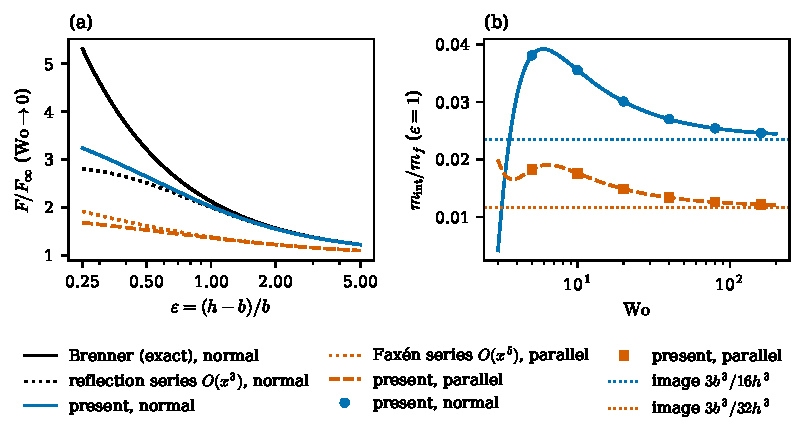
\includegraphics[width=0.85\textwidth]{figures/fig2_validation.pdf}
  \caption{Validation for a rigid sphere near a rigid wall. (a) Steady wall correction against Brenner's exact
  solution~\cite{brenner1961slow} and the classical reflection series (normal), and against Faxén's series (parallel).
  (b) Wall-induced added mass at $\varepsilon=1$ against the inviscid image values of \cref{prop:inviscid}.}
  \label{fig:validation}
\end{figure*}

\Cref{tab:validation} shows that the sphere solver reproduces the exact unsteady drag of a rigid sphere to all
printed digits. It also reproduces the Debye--Bueche--Brinkman drag of a porous sphere; the residual difference of
$<10^{-4}$ is the $O(\Wo)$ unsteady correction at $\Wo=10^{-4}$. \Cref{fig:validation}(a) compares the steady wall
correction with Brenner's exact series~\cite{brenner1961slow}. The dipolar closure follows the classical reflection
series through $O(x^3)$, as expected from \cref{rem:accuracy}. Its error relative to the exact solution is $5.1\%$ at
$\varepsilon=1$, $0.9\%$ at $\varepsilon=2$ and $<0.3\%$ for $\varepsilon\ge3$ in normal motion. Parallel motion is more accurate: it differs by $1.5\%$ from Faxén's fifth-order series at $\varepsilon=1$, because
the leading neglected coefficient is smaller. At $\varepsilon=0.5$
the error grows to $18\%$ (normal), confirming that the lubrication regime needs higher multipoles.
\Cref{fig:validation}(b) shows the high-frequency check. The wall-induced added mass decreases monotonically towards
the image values $3/(16h^3)=0.0234$ (normal) and $3/(32h^3)=0.0117$ (parallel) of \cref{prop:inviscid}: at $\Wo=160$ the
present values are $0.0246$ and $0.0122$. The remaining $5\%$ comes from higher image reflections, which the closure
retains, and from the $O(\Wo^{-1})$ boundary layers. The model therefore captures both ends of the frequency range.

\subsection{Rigid sphere: from a rigid wall to a permeable layer}\label{sec:rigid_results}

\begin{figure*}[t]
  \centering
  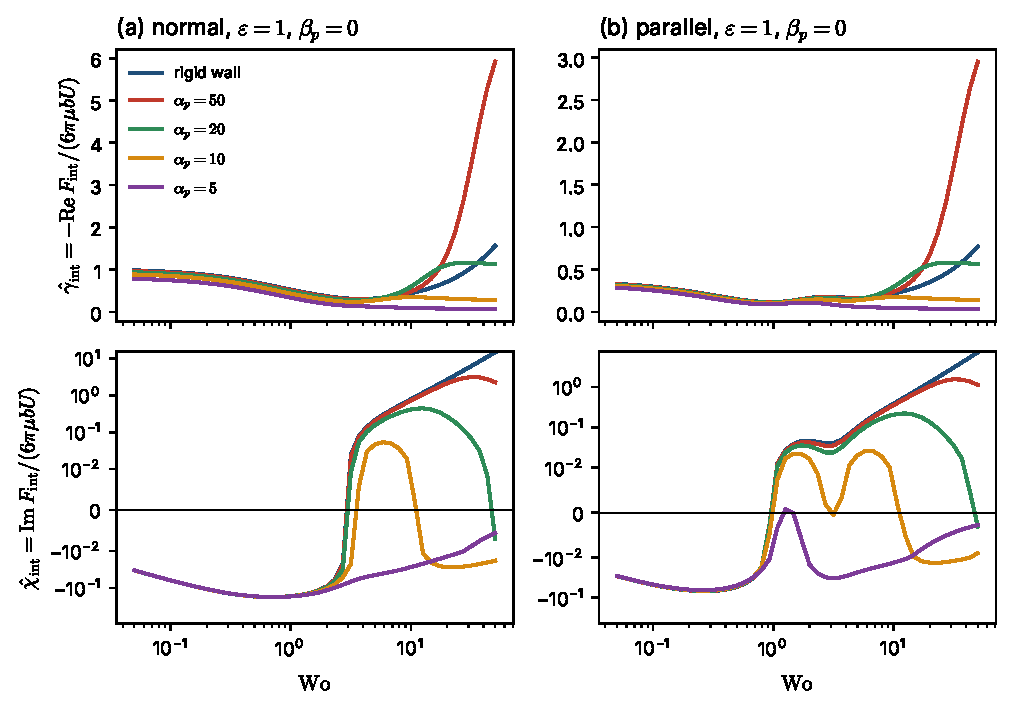
\includegraphics[width=0.85\textwidth]{figures/fig3_spectra_alphap.pdf}
  \caption{Interaction spectra of a rigid sphere at $\varepsilon=1$, $\beta_p=0$, for a rigid wall and layers with
  $\alpha_p=50,20,10,5$. Top: wall-induced damping $\hat\gamma_{\rm int}$. Bottom: reactive coefficient
  $\hat\chi_{\rm int}=\omega m_{\rm int}/(6\pi\mu b)$ (symmetric-log axis); its sign is that of $m_{\rm int}$. (a) Normal,
  (b) parallel oscillation.}
  \label{fig:spectra}
\end{figure*}

\Cref{fig:spectra} shows the wall-induced damping and reactive force as functions of $\Wo$. Near a rigid wall (blue)
the damping falls from its steady value $\hat\gamma_{\rm int}=0.98$ (normal) to a minimum of $0.31$ at $\Wo\approx3.7$,
then rises again, because the Stokes layer that forms on the wall dissipates more energy as $\Wo$ grows. The reactive
part is negative for $\Wo<\Wo_c=2.92$ and positive above it (normal); for parallel oscillation the crossover is at
$\Wo_c=0.955$. The negative branch has a simple interpretation. In unbounded fluid the Basset memory term
$-6\pi\lambda$ contributes a positive reactive force $6\pi\Wo/\sqrt2$, carried by vorticity that diffuses to distances
$|\lambda_f|^{-1}\gg h$ when $\Wo\ll1$. The wall truncates this diffusion, so it removes part of the memory force,
which appears as a negative added mass. Once $|\lambda_f|^{-1}\lesssim h$ the vorticity no longer reaches the wall,
and the reactive interaction is dominated by the potential image of \cref{prop:inviscid}, which is positive. With
\cref{rem:sign}, this reproduces the change of sign of the AFM resonance-frequency shift reported by Zhang
\emph{et al.}~\cite{zhang2023unsteady}.

A permeable layer changes this picture in three ways. First, in the steady limit the layer lets fluid escape through
the interface, so the damping is smaller: $\hat\gamma_{\rm int}(\Wo\to0)=0.94$, $0.89$ and $0.78$ for $\alpha_p=20$, $10$
and $5$ (normal). Second, at high frequency the reactive force does not keep growing. It peaks and then changes sign a
second time, because the layer becomes transparent to the oscillatory disturbance (\cref{rem:transparent}). Third, for
$\alpha_p=5$ the reactive force stays negative at all frequencies: the window of positive added mass has disappeared.
At $\Wo\approx\alpha_p$ the damping also shows a pronounced maximum, e.g.\ $\hat\gamma_{\rm int}=5.9$ at $\Wo=50$ for
$\alpha_p=50$, which is four times the rigid-wall value. This is the frequency at which the Stokes-layer thickness
matches the Brinkman screening length, so the oscillatory flow penetrates the layer and does work against its Darcy
drag. A rigid wall has no such dissipation channel.

\subsection{Crossover map: a frequency fingerprint of layer permeability}\label{sec:woc_results}

\begin{figure*}[t]
  \centering
  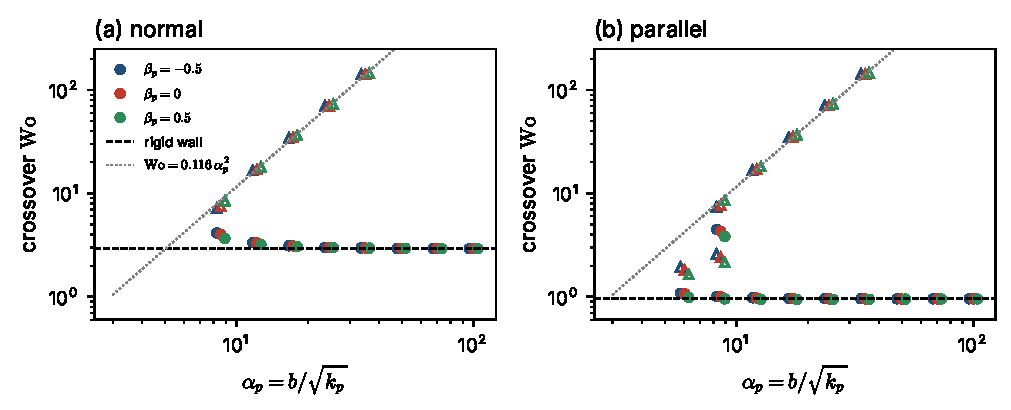
\includegraphics[width=0.85\textwidth]{figures/fig4_Woc_alphap.pdf}
  \caption{All crossover Womersley numbers of $m_{\rm int}$ against layer permeability at $\varepsilon=1$, for
  $\beta_p=-0.5,0,0.5$ (markers slightly offset horizontally). Filled circles: upward crossovers $\Wo_c^{\uparrow}$;
  open triangles: downward crossovers $\Wo_c^{\downarrow}$. Dashed: rigid-wall value. Dotted: fit
  $\Wo_c^{\downarrow}=0.116\,\alpha_p^2$. Upper crossovers above the scanned range ($\Wo\le\max(150,2.5\alpha_p)$) are not
  shown. (a) Normal, (b) parallel oscillation.}
  \label{fig:woc_ap}
\end{figure*}

\Cref{fig:woc_ap} collects all crossovers. Three features stand out.

\emph{(i) The lower crossover rises as the layer becomes more permeable.} For normal oscillation with $\beta_p=0$,
$\Wo_c^{\uparrow}=2.92$ (rigid wall), $2.96$ ($\alpha_p=35$), $3.10$ ($\alpha_p=17$) and $4.01$ ($\alpha_p=8.6$). The
shift is monotonic and becomes steep as $\alpha_p$ approaches about $10$, which is where the method is most sensitive.

\emph{(ii) An upper crossover scales as $\alpha_p^2$.} The downward crossover follows
$\Wo_c^{\downarrow}\approx0.116\,\alpha_p^2$ at $\varepsilon=1$: a least-squares fit gives exponent $2.08$, and
$\Wo_c^{\downarrow}/\alpha_p^2$ lies within $0.112$--$0.116$ for $\alpha_p\ge12$. The scaling is quadratic, not the naive $\Wo\sim\alpha_p$
suggested by \cref{eq:lambdas_nd}. In dimensional form it states that the viscous penetration depth at the upper
crossover is $\sqrt{\mu/\rho\omega}\approx8.6\,k_p/b$: the layer becomes transparent once the oscillatory boundary
layer is thinner than a length that combines the pore scale $\sqrt{k_p}$ with the ratio $\sqrt{k_p}/b$. For a probe of
known size, the upper crossover therefore measures $k_p$ directly. \TODO{authors: consider an asymptotic derivation of the prefactor $0.116$
and of its $\varepsilon$ dependence.}

\emph{(iii) The positive-added-mass window closes.} Below a threshold permeability no crossover exists in the scanned range, and the wall-induced added mass is negative
at all frequencies. The window closes between $\alpha_p=6.1$ and $8.6$ for normal oscillation, and between $4.3$ and
$6.1$ for parallel oscillation. For parallel oscillation near the threshold ($\alpha_p=8.6$) the window splits into two,
with four crossovers.

The stress jump $\beta_p$ has a weaker, systematic effect. A positive $\beta_p$, which increases the tangential momentum
transfer into the layer, lowers $\Wo_c^{\uparrow}$ (e.g.\ $3.64$ vs.\ $4.14$ for $\beta_p=0.5$ and $-0.5$ at
$\alpha_p=8.6$) and raises $\Wo_c^{\downarrow}$ slightly, so it widens the window. Its influence fades for
$\alpha_p\gtrsim30$.

\emph{Implication for microrheology.} A frequency sweep of the near-wall force of a colloidal probe at fixed $\varepsilon$
measures up to two crossovers. Each is a monotonic function of $\alpha_p$ in a different range: $\Wo_c^{\uparrow}$ is
sensitive for $\alpha_p\lesssim30$, and $\Wo_c^{\downarrow}$ for larger $\alpha_p$. Together they provide a non-contact
estimate of the layer permeability, for example to monitor degradation of the glycocalyx, which increases $k_p$.
\TODO{authors: map to dimensional AFM frequencies for a $b=5$--$20\,\mu$m probe in water and $k_p$ values from the
glycocalyx literature.}

\subsection{Steady limit}\label{sec:steady_results}
\begin{figure}[t]
  \centering
  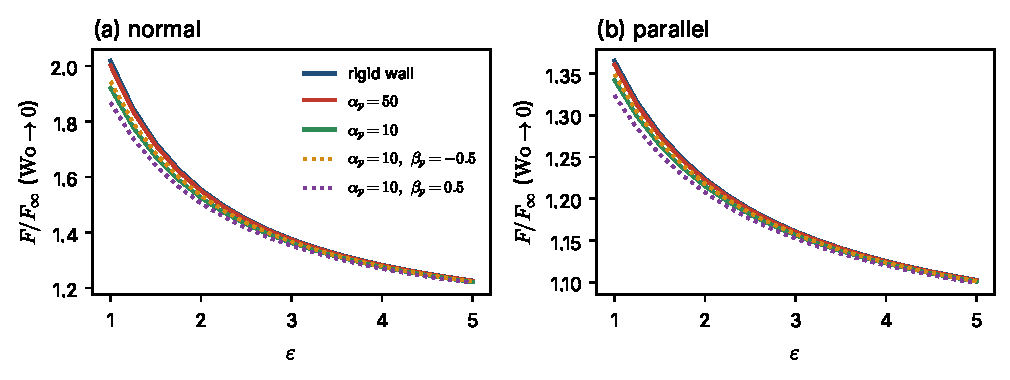
\includegraphics[width=\linewidth]{figures/fig6_steady.pdf}
  \caption{Steady ($\Wo\to0$) resistance of a rigid sphere against gap, for a rigid wall and for layers with
  $\alpha_p=50$ and $10$ and stress jumps $\beta_p=\pm0.5$. (a) Normal, (b) parallel.}
  \label{fig:steady}
\end{figure}
\Cref{fig:steady} shows the zero-frequency limit, where our formulation reduces to the problem of
Ref.~\onlinecite{faltas2021axisymmetric} (for normal motion) and extends it to parallel motion. Permeability lowers the
resistance, at $\varepsilon=1$ from $2.018$ (rigid wall) to $1.921$ ($\alpha_p=10$, normal) and from $1.365$ to $1.342$
(parallel). A positive $\beta_p$ lowers the resistance further ($1.867$ for
$\beta_p=0.5$) and a negative one raises it ($1.943$). All curves merge for $\varepsilon\gtrsim4$. Compared with the
unsteady crossovers, which shift by tens of per cent, the steady drag changes by only a few per cent. A frequency
sweep is therefore a far more sensitive probe of the layer than a steady drag measurement.

\subsection{Soft particles}\label{sec:soft_results}
\begin{figure*}[t]
  \centering
  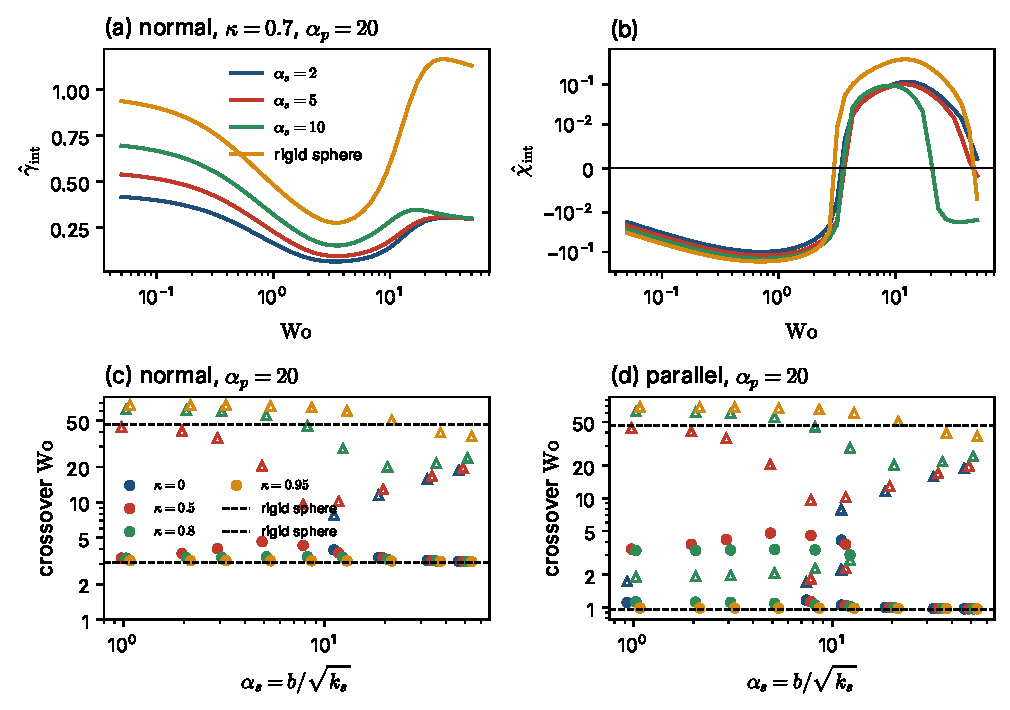
\includegraphics[width=0.85\textwidth]{figures/fig5_soft_particle.pdf}
  \caption{Soft core--shell particles near a glycocalyx-like layer ($\alpha_p=20$, $\beta_p=0$, $\varepsilon=1$).
  (a,b) Spectra for $\gamma=0.7$ and $\alpha_s=2,5,10$ against a rigid sphere (normal). (c,d) All crossover Womersley
  numbers against shell permeability for $\gamma=0,0.5,0.8,0.95$ (circles: upward; triangles: downward); dashed: rigid
  sphere.}
  \label{fig:soft}
\end{figure*}

\Cref{fig:soft}(a) shows that a permeable shell substantially reduces the wall-induced damping. For $\gamma=0.7$ the
steady value falls from $0.94$ (rigid) to $0.70$, $0.54$ and $0.42$ for $\alpha_s=10$, $5$ and $2$, and the minimum near
$\Wo\approx3.5$ falls from $0.28$ to $0.07$. Fluid passes through the shell instead of being squeezed out of the gap.
The high-frequency damping peak caused by the layer persists, but it is weaker because the scattered field is weaker.
The reactive part [\cref{fig:soft}(b)] keeps its crossover at $\Wo\approx3$--$4$, while its positive maximum is
reduced by a factor of about four.

The crossover maps [\cref{fig:soft}(c,d)] show a strong dependence on particle structure:
\begin{itemize}
\item \emph{Thin shells} ($\gamma=0.95$) behave like rigid spheres: $\Wo_c^{\uparrow}\approx3.18$ (normal) and $0.99$
      (parallel), independent of $\alpha_s$.
\item \emph{Homogeneous porous particles} ($\gamma=0$) lose the crossover in normal oscillation for $\alpha_s\le8$, so
      their wall-induced added mass is negative at all frequencies. For larger $\alpha_s$ the window reappears, with
      $\Wo_c^{\uparrow}=3.94$ at $\alpha_s=12$, decreasing towards the rigid value.
\item \emph{Intermediate cores} ($\gamma=0.5$) show a non-monotonic $\Wo_c^{\uparrow}(\alpha_s)$ with a maximum of $4.6$
      at $\alpha_s=5$ (normal). In parallel oscillation the low crossover near $\Wo\approx1$ disappears for
      $\alpha_s\le5$, and the first crossover jumps to $\Wo=3.4$--$4.8$. For $\gamma=0.8$ and $\alpha_s\le12$, parallel
      oscillation has two separate positive windows (four crossovers).
\end{itemize}
The upper crossover $\Wo_c^{\downarrow}$ also depends on the particle. It falls from $46$ (rigid sphere) to
$8$--$20$ for homogeneous porous particles and for $\gamma=0.5$ with $\alpha_s\ge8$. A weaker scattered field is
cancelled earlier by the transparency of the layer. \TODO{authors: confirm this interpretation.}

\emph{Implication for carriers.} A permeable shell lowers the near-wall damping by up to a factor of four and removes
the positive-added-mass window. Such a particle therefore experiences less resistance when driven near a mucus layer,
which supports the use of soft, PEG-like shells in mucus-penetrating carriers~\cite{pangeni2023airway}. The core slip
$\hat\ell_c$ is included in the model but has a weaker effect when the shell is permeable. \TODO{authors: add a panel
or table varying $\hat\ell_c$ and $\beta_s$ if the reviewers ask.}

\subsection{Acoustofluidic contrast between cell-like particles}\label{sec:acoustic_results}
\begin{figure*}[t]
  \centering
  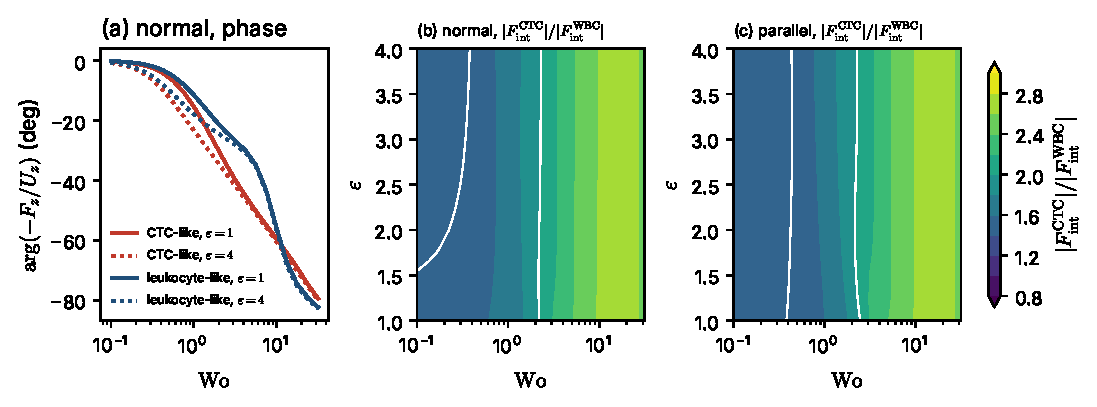
\includegraphics[width=0.9\textwidth]{figures/fig7_acoustic_contrast.pdf}
  \caption{CTC-like ($\gamma=0.9$, $\alpha_s=20$) against leukocyte-like ($\gamma=0.7$, $\alpha_s=5$) particles of equal outer
  radius near an endothelial-like layer ($\alpha_p=20$, $\beta_p=0$). (a) Phase of the total resistance at
  $\varepsilon=1$ and $4$ (normal). (b,c) Ratio of the magnitudes of the wall-induced forces (white contours: $1$, $1.5$,
  $2$).}
  \label{fig:acoustic}
\end{figure*}

As an illustration for acoustofluidic sorting~\cite{wu2019acoustofluidic,hossein2023review}, \cref{fig:acoustic}
compares two particles of the same outer radius, a stiffer CTC-like particle and a softer leukocyte-like particle. The
parameters in \cref{tab:params} are representative, not fitted to specific cell lines. The phase of the total resistance
[\cref{fig:acoustic}(a)] differs by up to $13^\circ$ near $\Wo\approx3$ and by less than $1^\circ$ for $\Wo\lesssim0.3$. The
wall-induced force of the CTC-like particle is $1.4$--$2.7$ times larger [\cref{fig:acoustic}(b,c)]. The ratio depends
mainly on $\Wo$ and only weakly on $\varepsilon$, and it is largest for $\Wo\gtrsim5$. The wall-induced force is a
significant fraction of the total only close to the layer: at $\varepsilon=1$, $|F_{\rm int}|/|F_\infty|=0.78$ (normal)
at $\Wo=0.1$, but $0.04$ at $\Wo=10$. Near-wall sorting by softness therefore works best at moderate frequencies,
$\Wo=O(1)$, where both the phase contrast and the near-wall force are appreciable. Most of the force contrast at
higher $\Wo$ comes from the unbounded resistance itself. \TODO{authors: couple to an acoustic radiation-force model to
predict trajectory separation; cite device-specific parameters.}

\subsection{Insights, limitations and sensitivity}\label{sec:limitations}
\begin{itemize}
\item \emph{Main insight.} Permeability introduces a new frequency scale into the near-wall unsteady force. The
      viscous diffusion time $\rho h^2/\mu$ sets the familiar crossover $\Wo_c^{\uparrow}=O(1)$. The layer adds an
      upper crossover $\Wo_c^{\downarrow}\approx0.116\,\alpha_p^2$ at which it becomes transparent. When the two meet
      ($\alpha_p\approx6$--$9$ normal, $4$--$6$ parallel, at $\varepsilon=1$), the positive-added-mass regime
      disappears.
\item \emph{Accuracy.} The dipolar closure is accurate to $5\%$ (normal) and $1.5\%$ (parallel) at $\varepsilon=1$ and
      much better beyond (\cref{tab:validation}). We expect crossover locations to be less affected than force magnitudes, because the neglected $l\ge2$ terms mainly
rescale the interaction. \TODO{authors: confirm with a multipole or FEM
      computation at $\varepsilon=1$.}
\item \emph{Model limitations.} The model assumes a rigid porous matrix, a half-space layer, no particle rotation, equal
      Brinkman and fluid viscosities, and no lubrication. Poroelastic glycocalyx deformation~\cite{batalha2026elasto} and
      finite layer thickness are expected to modify the high-frequency branch.
\item \emph{Sensitivity.} The results are insensitive to the quadrature (relative changes $<10^{-13}$). The Richardson extrapolation of the steady limit removes the $O(\Wo)$ unsteady correction. The
      extrapolated values agree with Brenner's exact solution to three to four digits for $\varepsilon\ge3$
      (\cref{tab:validation}).
\end{itemize}

\section{Conclusions}\label{sec:conclusion}
% GUIDE BULLETS -- the authors turn these into prose.
\begin{itemize}
  \item \textbf{Summary:} semi-analytical theory for the oscillatory force on a soft core--shell particle near a
        Brinkman half-space with stress jump. It combines an exact $l=1$ sphere response, an exact Fourier reflection and a
        self-consistent dipolar closure, and is validated against exact, steady and inviscid limits.
  \item \textbf{Rigid reference:} near a rigid wall, the wall-induced added mass changes sign once, at
        $\Wo_c\approx2.9$ (normal) and $\approx0.95$ (parallel) for $\varepsilon=1$. This is consistent with the
        frequency-shift crossover of Ref.~\onlinecite{zhang2023unsteady}, and $m_{\rm int}$ approaches the inviscid image
        values at high $\Wo$.
  \item \textbf{Permeable layer:} a finite $\alpha_p$ raises the lower crossover and adds an upper crossover where the
        layer becomes transparent to the oscillatory disturbance. The positive-added-mass window shrinks as
        $\alpha_p$ decreases and disappears below a threshold ($\alpha_p\approx6$--$9$ normal, $4$--$6$ parallel, at $\varepsilon=1$); the upper crossover follows $\Wo_c^{\downarrow}\approx0.116\,\alpha_p^2$. The
        stress jump $\beta_p$ shifts these boundaries only weakly.
  \item \textbf{Soft particle:} shell permeability and core size shift $\Wo_c$ non-monotonically. Highly porous
        particles ($\gamma\to0$, small $\alpha_s$) lose the crossover in normal oscillation, and intermediate core
        sizes produce re-entrant crossovers in parallel oscillation.
  \item \textbf{Biomedical takeaways:} (i) the frequency positions of the crossovers form a non-contact fingerprint of
        layer permeability (glycocalyx degradation, mucus hydration); (ii) cell-like particles of different softness
        differ in near-wall force amplitude and phase, which is exploitable in acoustofluidic sorting; (iii) soft,
        permeable shells reduce near-wall damping, which favours mucus-penetrating carriers.
  \item \textbf{Limitations:} dipolar closure accurate for $\varepsilon\gtrsim1$ (no lubrication); rigid stationary
        porous matrices; no particle rotation; layer modelled as a half-space; Brinkman viscosities set equal to $\mu$.
  \item \textbf{Future work:} full multipole collocation for $\varepsilon<1$; finite-thickness layers on a substrate;
        poroelastic layers; free rotation; comparison with colloidal-probe AFM on glycocalyx-mimicking brushes.
\end{itemize}


\appendix
\section{Linear system for the core--shell particle}\label{app:sphere}
Each term of \cref{eq:fields} has velocity, pressure and traction amplitudes $(\mathcal U,\mathcal V,\mathcal P,\mathcal
S_{rr},\mathcal S_{r\theta})$ as defined in \cref{sec:sphere}. For the vortical terms they follow from
\cref{eq:vort_radial} with $g=\mathcal K_j$ or $\mathcal I_j$ and $\mathcal P=0$. For the potential terms, with the
pressure coefficients $c_j$ of \cref{lem:decomp}, they are
\begin{align*}
  \be:&\quad \mathcal U=1,\ \mathcal V=-1,\ \mathcal P=c_j\,r,\\
  \nabla(\be\cdot\nabla r^{-1}):&\quad \mathcal U=2r^{-3},\ \mathcal V=r^{-3},\ \mathcal P=-c_j\,r^{-2}.
\end{align*}
The rigid part $\be$ of \cref{eq:field_shell} carries the pressure $i\Wo^2\be\cdot\bx$, so its amplitudes at $r=1$ are
$\mathcal U=1$, $\mathcal V=-1$, $\mathcal S_{rr}=-i\Wo^2$ and $\mathcal S_{r\theta}=0$. Let a tilde denote the shell
field without its rigid part, and let shell tractions be computed with $\mu_s/\mu$. The conditions
\cref{eq:bc_core,eq:bc_shell} then read
\begin{align*}
  r=\kappa:&\quad \tilde{\mathcal U}^{(2)}=0,\qquad \tilde{\mathcal V}^{(2)}-\frac{\hat\ell_c}{\mu_s/\mu}\,\tilde{\mathcal S}^{(2)}_{r\theta}=0,\\
  r=1:&\quad \mathcal U^{(1)}=\mathcal U^{(2)},\quad \mathcal V^{(1)}=\mathcal V^{(2)},\quad
  \mathcal S^{(1)}_{rr}=\mathcal S^{(2)}_{rr},\quad
  \mathcal S^{(2)}_{r\theta}-\mathcal S^{(1)}_{r\theta}=\beta_s\alpha_s\left(\mathcal V^{(1)}+1\right).
\end{align*}
The kernels are rescaled to avoid overflow when $|\lambda_s|$ or $|\lambda|$ is large: $\mathcal K_s(r)e^{\lambda_s\kappa}$,
$\mathcal I_s(r)e^{-\lambda_s}$, $\mathcal K_f(r)e^{\lambda}$ and $\mathcal I_f(r)e^{-\lambda}$. The scaling factors are
removed from the coefficients after the solve. For a homogeneous porous particle ($\kappa=0$, $\beta_s=0$,
$\mu_s=\mu$, $\Wo\to0$) the solver reproduces the Debye--Bueche--Brinkman drag ratio
$\Omega=2\alpha_s^2(1-\alpha_s^{-1}\tanh\alpha_s)/[2\alpha_s^2+3(1-\alpha_s^{-1}\tanh\alpha_s)]$
(\cref{tab:validation}).

\section{Interface system in Fourier space}\label{app:interface}
For a plane mode $\propto e^{i\bk\cdot\bx_\parallel+sz}$ with velocity amplitude $\hat\bu$ and pressure amplitude
$\hat p$, the tractions at $z=0$ in a medium of viscosity $\mu_j$ are
\begin{equation*}
  \hat\sigma_{xz}=\mu_j\left(s\hat u_x+ik_x\hat u_z\right),\quad
  \hat\sigma_{yz}=\mu_j\left(s\hat u_y+ik_y\hat u_z\right),\quad
  \hat\sigma_{zz}=-\hat p+2\mu_js\hat u_z .
\end{equation*}
The potential mode has $\hat\bu=(ik_x,ik_y,s)$ and $\hat p=c_j$, with $s=-k$ (reflected) or $s=k$ (transmitted). The
poloidal mode has $\hat\bu=(ik_xs,ik_ys,k^2)$ and the toroidal mode $\hat\bu=(ik_y,-ik_x,0)$, both with $\hat p=0$ and
with $s=-q$ (reflected) or $s=q_p$ (transmitted). With superscripts ``inc'', $R$ and $T$ for the incident, reflected and
transmitted fields, the six rows of \cref{eq:interface_system} are
\begin{align*}
  &\hat\bu^{R}-\hat\bu^{T}=-\hat\bu^{\rm inc}\quad(3\ \text{rows}),\qquad
  \hat\sigma^{R}_{zz}-\hat\sigma^{T}_{zz}=-\hat\sigma^{\rm inc}_{zz},\\
  &\hat\sigma^{T}_{\tau z}-\hat\sigma^{R}_{\tau z}-\beta_p\alpha_p\hat u^{R}_\tau
   =\hat\sigma^{\rm inc}_{\tau z}+\beta_p\alpha_p\hat u^{\rm inc}_\tau\quad(\tau=x,y).
\end{align*}
The columns of $\mathsf A$ are normalised to unit Euclidean norm before solving, which removes the $O(k)$ degeneracy of
the mode vectors as $k\to0$. For a rigid wall the system reduces to $\hat\bu^R=-\hat\bu^{\rm inc}$.


\begin{acknowledgments}
\TODO{funding and acknowledgements}
\end{acknowledgments}

\section*{Data Availability Statement}
{\sloppy The code that generates every figure and table (\texttt{code/osc\_solver.py},\linebreak[1] \texttt{code/make\_results*.py},
\texttt{figures/make\_figures.py}) is \TODO{to be deposited in a public repository; give the link}.\par}

\bibliography{references}

\end{document}
